\documentclass{jarticle}

% 画像
\usepackage[dvipdfmx]{graphicx}
% リンク
\usepackage[dvipdfmx]{hyperref}
% URL
\usepackage{url}
% 目次
\usepackage{pxjahyper}
% フォント関連
\usepackage{amsfonts}
\usepackage{amsmath, amssymb}
\usepackage{mathrsfs}	% for \mathscr{}
\usepackage{bm}
\usepackage{here}
\usepackage{color}
\usepackage[super]{cite}
\usepackage{ascmac}
\usepackage{multirow}
\usepackage{booktabs}
% ソースコード表示のための設定
\usepackage{listings,jlisting}

\renewcommand\citeform[1]{[#1]}

\lstset{
  basicstyle={\ttfamily},
  identifierstyle={\small},
  commentstyle={\smallitshape},
  keywordstyle={\small\bfseries},
  ndkeywordstyle={\small},
  stringstyle={\small\ttfamily},
  frame={tb},
  breaklines=true,
  columns=[l]{fullflexible},
  numbers=left,
  xrightmargin=0zw,
  xleftmargin=3zw,
  numberstyle={\scriptsize},
  stepnumber=1,
  numbersep=1zw,
  lineskip=-0.5ex
}

% 余白の設定
\usepackage[margin=20truemm]{geometry}

\begin{document}
\title{1年生実習 第3週}
\author{B5研究室}
\date{2024年7月3日}
\maketitle

\section{SVM(サポートベクターマシン)}
本日使用するモデルは,SVM(サポートベクターマシン)です.
SVMは,分類問題において高い性能を発揮することが知られています.

それでは,SVMの基本的な原理について見てみましょう.
分類対象のデータとして,図\ref{fig:svm_data}のような2クラスの2次元データを考えます.

\begin{figure}[H]
  \centering
  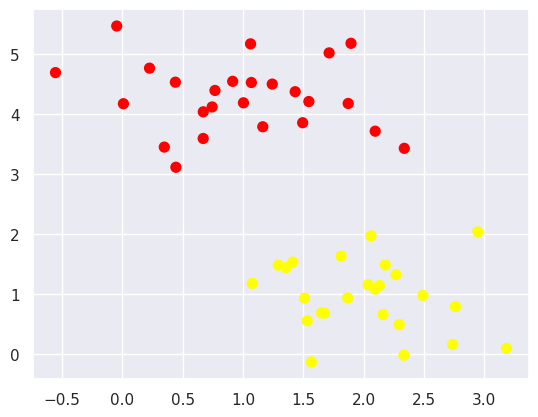
\includegraphics[width=10cm]{fig/svm_data.png}
  \caption{SVMのデータ}
  \label{fig:svm_data}
\end{figure}

赤色と黄色の2クラスのデータを分類するために,2つのクラスを分離する直線を見つけることが目標です.
このとき,どのようにして直線を引くことができるでしょうか?
次のページに進む前に\textbf{定規で試しに線を引いてみてください.}
\newpage

クラスを分割する線の例として,図\ref{fig:svm_lines}のような線が考えられます.

\begin{figure}[H]
  \centering
  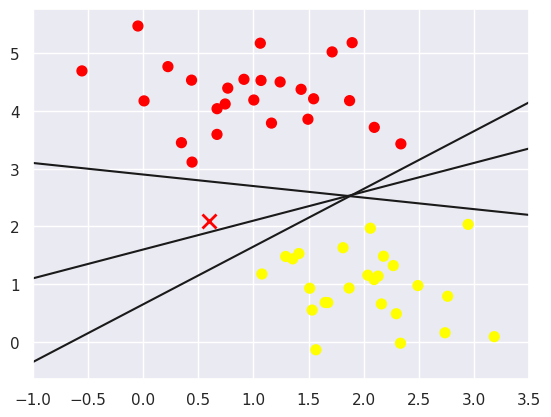
\includegraphics[width=10cm]{fig/svm_lines.png}
  \caption{SVMの直線}
  \label{fig:svm_lines}
\end{figure}

これらの線は,赤色と黄色の線をうまく分割できています.
しかしながら,どの線を境界とするかによって,図\ref{fig:svm_lines}の赤い$\times$で示したデータのクラスが変わってしまいます.
「クラス間に線を引く」という考え方は直感的で簡単ですが,実際の問題を解くためにはまだ不十分であることがわかります.

そこで登場するのが,マージン最大化という考え方です.
マージンとは,クラス間の最も近いデータ点と境界線の距離のことです.
クラス間の最も近いデータ点のことをサポートベクターと呼びます.
図\ref{fig:svm_lines}の線におけるマージンを可視化した図を図\ref{fig:svm_margin}に示します.

\begin{figure}[H]
  \centering
  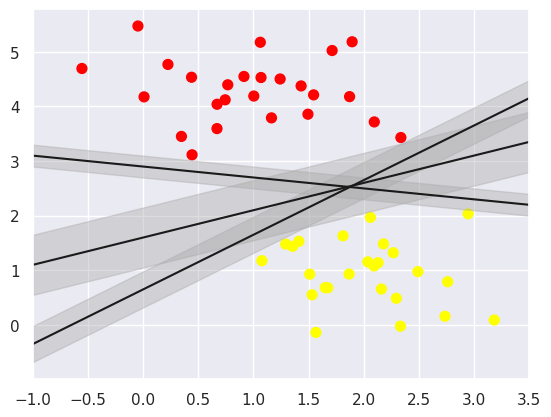
\includegraphics[width=10cm]{fig/svm_margin.png}
  \caption{SVMのマージン}
  \label{fig:svm_margin}
\end{figure}

図\ref{fig:svm_margin}の例では,中央の線が最も大きなマージンを持っています.
しかしながら,この線は最大のマージンを持っているわけではありません.
SVMでは,このようなマージンを最大化する直線を見つけることができます.
SVMによって見つけられた直線は,図\ref{fig:svm_sv}のようになります.

\begin{figure}[H]
  \centering
  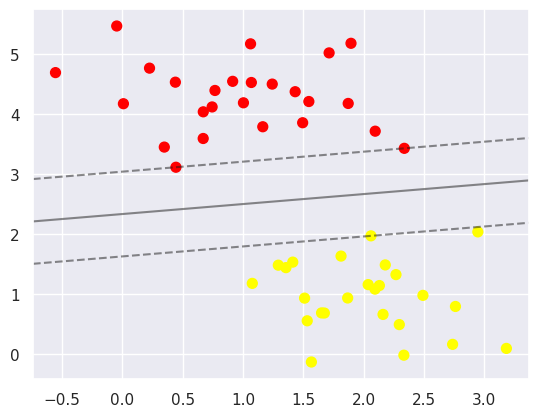
\includegraphics[width=10cm]{fig/svm_support_margin.png}
  \caption{SVMのサポートベクターとマージン}
  \label{fig:svm_sv}
\end{figure}

図\ref{fig:svm_sv}の直線は,サポートベクターによって定義されるマージンを最大化する直線です.

では,データ数が変わった場合はどうなるでしょうか?
図\ref{fig:svm_data2}に,データ数が変化した場合のSVMの分割例を示します.

\begin{figure}[H]
  \centering
  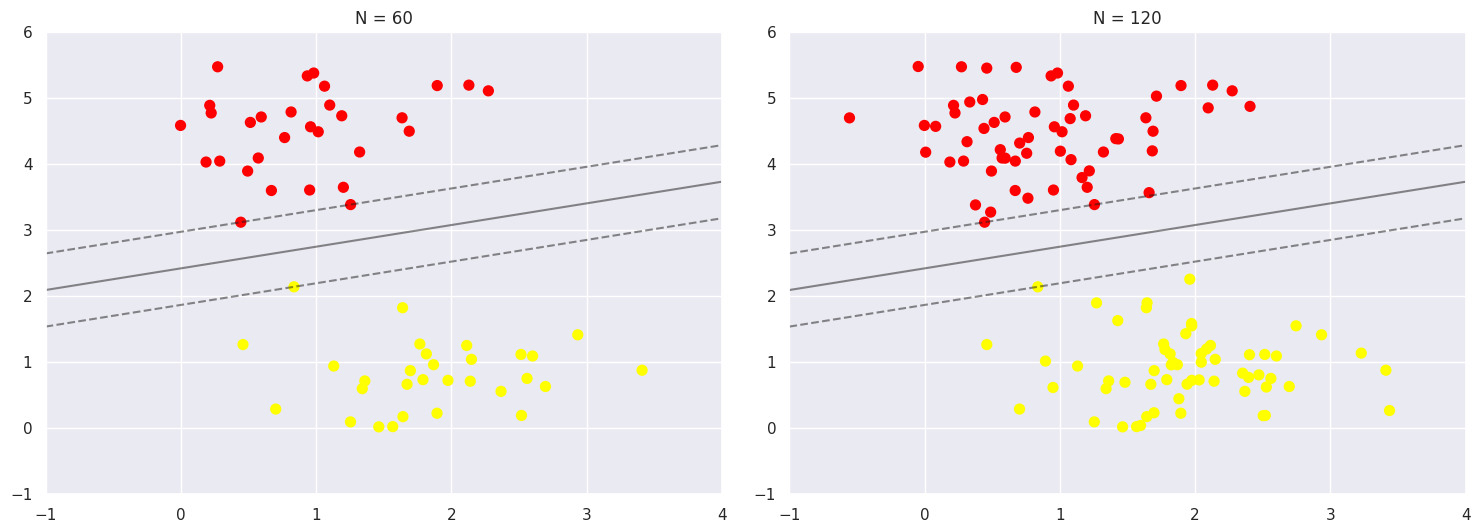
\includegraphics[height=6.1cm]{fig/svm_diff_sample_amount.png}
  \caption{データ数が変化した場合の決定境界(右:60点,左:120点)}
  \label{fig:svm_data2}
\end{figure}

SVMは境界線から遠いデータに影響されず,サポートベクターのみを用いて境界線を引いていることがわかります.
このような,境界から離れたデータに対する影響が少ない性質が,SVMの特徴の一つです.

ここまで見てきたデータは,決定境界が直線の場合のデータです.
直線で分割できるデータのことを,線形\footnote{``線形"という用語は,様々な場面で登場しますが,基本的には,直線で表せる関係を意味します.}分離可能なデータといいます.
では,境界線が直線ではない場合はどうなるでしょうか?
図\ref{fig:not_linear}に,直線で分割できないデータを示します.

\begin{figure}[H]
  \centering
  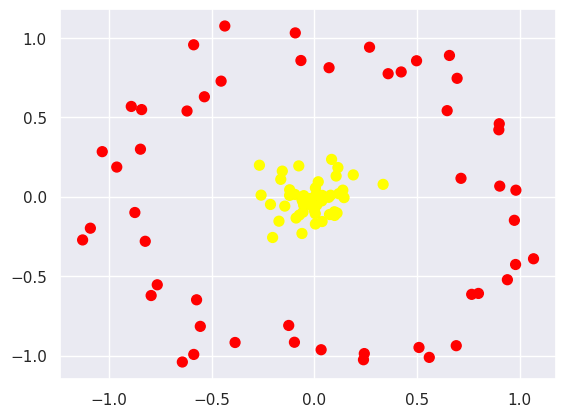
\includegraphics[width=10cm]{fig/svm_not_linear.png}
  \caption{直線で分割できないデータ}
  \label{fig:not_linear}
\end{figure}

図\ref{fig:not_linear}のデータを分割するために,図\ref{fig:not_linear}に高さ方向の次元を追加した3次元空間を考えてみましょう.
このとき,図\ref{fig:not_linear}のデータを3次元空間にプロットするための式として,次のような式が考えられます.

\begin{equation}\label{eq:kernel}
  r = e^{-(x^2 + y^2)}
\end{equation}

式(\ref{eq:kernel})は,2次元データ$(x, y)$を3次元データ$(x, y, r)$に変換する式です.
この関数は,原点が最も高い値を持ち,原点から離れるほど値が小さくなるような関数です.(図\ref{fig:RBF})
このような,距離に基づいて値が決まる関数のことを,放射基底関数(Radial Basis Function: RBF)といいます.

\begin{figure}[H]
  \centering
  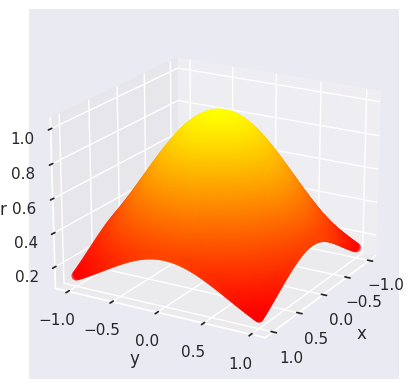
\includegraphics[width=10cm]{fig/RBF_function.png}
  \caption{RBF関数}
  \label{fig:RBF}
\end{figure}

では,RBF関数を用いて,図\ref{fig:not_linear}のデータを3次元空間にプロットしてみましょう.
図\ref{fig:3d_data}に,RBF関数を用いて3次元空間にプロットしたデータを示します.

\begin{figure}[H]
  \centering
  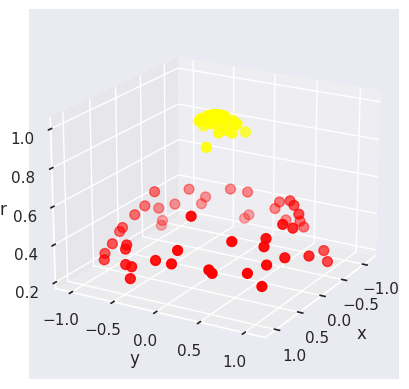
\includegraphics[width=10cm]{fig/SVM_RBF.png}
  \caption{RBF関数を用いて3次元空間にプロットしたデータ}
  \label{fig:3d_data}
\end{figure}

図\ref{fig:3d_data}を見れば,だいたい$r=0.7$となるあたりの平面で分割すればうまくいきそうだとわかります.
しかしながら,式\ref{eq:kernel}はたまたまうまくいっただけであり,(当たり前ですが)すべての場合でうまくいくわけではありません.
今回の例では3次元空間にデータをプロットしましたが,実際のデータはさらに高次元の空間にプロットされる場合がほとんどです.

今回のRBF関数のような,データを高次元空間に写像する関数をカーネルといいます.



RBF関数をにした,



詳細は割愛しますが,SVMでは,カーネルトリックという素晴らしい手法によりこの問題を解決しています.
カーネルトリックを使用することで,SVMは高次元空間での計算を効率的に行い,非線形なデータでも効果的に分離することができます.
SVMはカーネルトリックという手法の恩恵を受けている,ということだけ覚えておいてください.

話をデータの分類に戻します.図\ref{fig:svm_RBF}にRBF関数によって分類された結果を示します.

\begin{figure}[H]
  \centering
  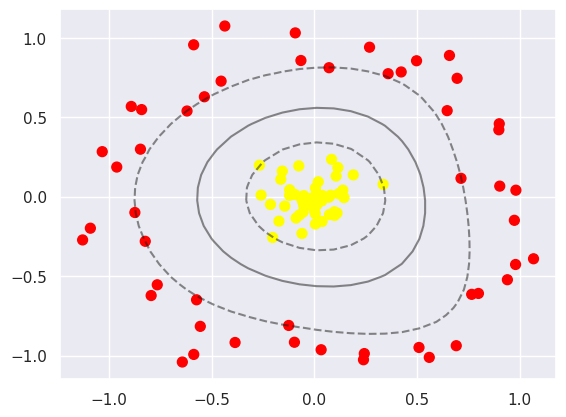
\includegraphics[width=10cm]{fig/svm_rbf_db.png}
  \caption{SVMの分類結果(RBF関数)}
  \label{fig:svm_RBF}
\end{figure}

線形に分割できなかったデータをRBF関数を用いて,マージンが最大となるようにうまく分割することができました.

SVMでは,高次元空間で分類を行うために,それぞれのデータの類似度を計算します.
この類似度を計算する関数のことをカーネル関数といいます.
RBF関数は,

RBF関数のような,データを高次元空間に写像する関数をカーネル関数といいます.
RBFカーネル以外にも,多項式カーネルやシグモイドカーネルなど,様々なカーネル関数が存在します.
カーネル関数を用いて,データを高次元空間に写像する手法のことをカーネル法といいます.
カーネル法を使用したSVMは,非線形なデータに対しても高い性能を発揮することが知られているため,頻繁に使用されます.


\section{機械学習によるデータ分類}
今週の実習では,先週の実習で皆さんから集めた手書き文字データを分類するための機械学習モデルを構築します.
現状のデータセットの状態は以下の通りです.

\begin{itemize}
  \item 取得文字: $ \bigcirc  \times $ の2文字
  \item 取得文字数: 3セット $ \times $ 10人の60文字
  \item データ長:最長のデータに合わせて引き伸ばし(M1の方で処理済)
  \item 座標軸:X, Y, Zの3軸
\end{itemize}

このデータセットを用いて,分類を行うための機械学習モデルを構築します.

今回の演習で使用するライブラリは,Scikit-learnです.
Scikit-learnは,Pythonで使用できる機械学習ライブラリの一つで,多くの機械学習モデルを提供しています.


\subsection{データの準備}
Pythonを用いてGoogle Driveから分類用データをダウンロードします.(ソースコード\ref{sc:download})

\begin{lstlisting}[caption=データのダウンロード, label=sc:download]
  # 分類するデータのダウンロード
  import gdown

  url = "https://drive.google.com/uc?id=1rcAg1R0rYLoeQ2ColX4BvM80u841qx5W"
  output = "data.zip"
  gdown.download(url, output, quiet=False) # Google Driveからdata.zipをダウンロード

  # ダウンロードしたデータを解凍
  !mkdir data
  !unzip -o data.zip -d data
  !rm data.zip
\end{lstlisting}

Jupyter Notebookでは,``!"を先頭につけることで,Linuxコマンドを実行することができます.
上記のコードでは,PythonコードでGoogle Driveからデータをダウンロードしたあと,Linuxコマンドを用いてZIPファイルを解凍(不要なファイルを削除)しています.

\subsection{データの分割}
今回使用するデータは実際に計測した数値データに前処理を適用したあとのデータです.
したがって,今回は正規化などの前処理は不要です.

分類器による学習のために,データを訓練データとテストデータに分割します.
分割する割合は,訓練データ:テストデータ = 8:2とします.(ソースコード\ref{sc:split})

\begin{lstlisting}[caption=データの分割, label=sc:split]
  from sklearn.model_selection import train_test_split # データ分割を行う関数のインポート

  # データの分割
  X_train, X_test, y_train, y_test = train_test_split(X, y, test_size=0.2, random_state=1234)
\end{lstlisting}

\begin{itembox}[l]{\textbf{ライブラリのインポート}}
  Pythonでは,様々な処理を行うための外部ライブラリが豊富に用意されています.
  ライブラリをインポートするためには,\texttt{import}文を用います.

  \begin{lstlisting}[caption={ライブラリのインポート}]
    import ライブラリ名 # ライブラリのインポート
    import ライブラリ名 as 別名 # ライブラリのインポート(別名をつける)
    from ライブラリ名 import 関数名 # ライブラリ内の特定の関数のみをインポート
    from ライブラリ名 import * # ライブラリ内の全ての関数をインポート(非推奨)
  \end{lstlisting}

\end{itembox}

\texttt{random\_state}は,データを分割する際の乱数のシードを指定する引数です.
\texttt{random\_state}を指定することで,データの分割を再現可能にすることができます.
再現性を確保しておくことは,実験結果の検証の際に非常に重要となります.
シードの値は任意で構いませんが,実験結果を再現するためには,同じ値を指定しておくことが一般的です.

\subsection{SVMによる分類}
データの分割が完了したら,SVMによる分類を行います.\
Scikit-learnのSVMを使用するためには,\texttt{SVC}クラスをインポートします.(ソースコード\ref{sc:svm})

\begin{lstlisting}[caption=SVMによる分類, label=sc:svm]
  from sklearn.svm import SVC # SVMのインポート

  # SVMのインスタンスを生成
  clf = SVC(kernel='linear', random_state=1234)

  # モデルの学習
  clf.fit(X_train, y_train)
\end{lstlisting}

SVCクラスには,いくつかの引数があります.
\texttt{kernel}は,カーネル関数を指定する引数です.
この例では,線形カーネルを使用しているため,\texttt{kernel='linear'}と指定しています.
他にも,多項式カーネル(\texttt{kernel='poly'})やRBFカーネル(\texttt{kernel='rbf'})など,様々なカーネル関数を指定することができます.

また,他の引数として,\texttt{C}や\texttt{gamma}などがあります.
これらのパラメータを調整することで,SVMの性能を向上させることができますが,今回はデフォルト値を使用します.

\subsection{予測と評価}
学習が完了したら,テストデータを用いて予測を行い,モデルの性能を評価します.
予測を行うためには,\texttt{predict}メソッドを使用します.(ソースコード\ref{sc:predict})

\begin{lstlisting}[caption=予測と評価, label=sc:predict]
  # テストデータを用いて予測
  y_pred = clf.predict(X_test)

  # モデルの評価
  from sklearn.metrics import accuracy_score, classification_report # 評価指標を計算する関数のインポート
  classification_report(y_test, y_pred) # 分類結果の表示
  accuracy = accuracy_score(y_test, y_pred) # 正解率の計算
  print(f"正解率: {accuracy:.2f}")

  # 分類結果の表示
  print(classification_report(y_test, y_pred))
\end{lstlisting}

分類結果を表示するために,\texttt{classification\_report}関数を使用しています.
classification\_report関数は,適合率(precision)や再現率(recall),F1スコアなどの評価指標を計算して表示します.
これらの指標はどのような意味を持つのでしょうか?

\subsubsection{混同行列}
適合率などの指標の話をする前に,混同行列について説明します.
混同行列は,予測結果と実際の結果まとめた表です.
混同行列は,表\ref{tb:confusion_matrix}のように表されます.

\begin{table}[H]
  \centering
  \caption{混同行列}
  \label{tb:confusion_matrix}
  \begin{tabular}{c|c|c c}\hline
    \multicolumn{2}{c}{} & \multicolumn{2}{|c}{予測値} \\
    \cline{3-4}
    \multicolumn{1}{c}{} &  & 陽性 & 陰性 \\
    \hline
    \multirow{2}{*}{実際の値} & 陽性 & TP & FN \\
    & 陰性 & FP & TN \\
    \hline
  \end{tabular}
\end{table}

混同行列には,真陽性(True Positive: TP),偽陽性(False Positive: FP),真陰性(True Negative: TN),偽陰性(False Negative: FN)の4つの要素があります.
真陽性は,実際に正であり,正と予測されたデータの数を示します.
偽陽性は,実際に負であるが,正と予測されたデータの数を示します.
真陰性は,実際に負であり,負と予測されたデータの数を示します.
偽陰性は,実際に正であるが,負と予測されたデータの数を示します.

\subsubsection{正解率,適合率,再現率,F1スコア}
正解率,適合率,再現率,F1スコアの4つの指標は,先述した混同行列を用いて計算されます.

各項目の計算式は以下の通りです.

\begin{itemize}
  \item 正解率(accuracy):$\frac{TP + TN}{TP + FP + FN + TN}$
  \item 適合率(precision):$\frac{TP}{TP + FP}$
  \item 再現率(recall):$\frac{TP}{TP + FN}$
  \item F1スコア:$\frac{2 \times \text{適合率} \times \text{再現率}}{\text{適合率} + \text{再現率}}$
\end{itemize}

正解率とは,全体のデータのうち,正しく分類されたデータの割合を示します.
適合率とは,正と予測されたものの中で実際に正であったものの割合を示します.
再現率とは,実際に正であったものの中で正と予測されたものの割合を示します.
F1スコアは,適合率と再現率の調和平均です.

モデルを評価するとき,正解率が高いモデルが良いモデルであるとは限りません.
正解率だけでモデルの性能を評価するのは危険です.
正解率だけの評価では不十分な例として,データの偏りがある場合が挙げられます.
筆跡から利き手を予測するモデルを作ることを考えてみます.
人口のだいたい90\%以上が右利きであると言われています.
したがって,筆跡を根拠としなくても,右利きと予測するだけで正解率が90\%以上になります.
しかしながら,このモデルは,左利きの人を全て右利きと予測してしまうため,実用的なモデルとは言えません.
このような場合,適合率や再現率などの指標を用いてモデルの性能を評価することが重要です.

では,適合率や再現率はどのような意味を持つのでしょうか?
例として,顧客のプロフィール情報からある商品を購入するかを予測するモデルを考えます.
このとき,適合率が表すのは,購入すると予測されたデータのうち,実際にその商品を購入したデータがどれくらいあるかということです.
適合率が低いことがわかった場合,購入すると予測されたデータのうち,実際に購入したデータが少ないことを示します.
この場合,購入すると予測されたデータのうち,実際に商品を購入しないデータが多いため,無駄な広告費用がかかったり,過剰発注をしてしまうなどの損失が発生することが想定されます.

一方,再現率が表すのは,実際にその商品を購入したデータのうち,購入すると予測されたデータがどれくらいあるかということです.
再現率が低い場合,実際に商品を購入したデータのうち,購入すると予測されたデータが少ないことを示します.
この場合,購入すると予測されたデータが少ないため,在庫が足りなくなってしまうことが想定されます.

これらの例からも分かるように,適合率と再現率はトレードオフの関係にあります.
適合率を高くするためには,購入すると予測されたデータを減らす必要があります.
一方で,再現率を高くするためには,実際に購入するデータを増やす必要があります.
このように,適合率と再現率はトレードオフの関係にあるため,どちらを重視するかによって,モデルの評価が変わってきます.

では,どのようにして適合率と再現率のバランスを取ればよいでしょうか?
適合率と再現率のバランスを評価するための指標がF1スコアです.
F1スコアは,適合率と再現率の調和平均で計算されます.
調和平均とは,データの各数値の逆数で平均を取り,その平均の逆数を取ることで求められる平均のことです.
算術平均(=合計$\div$個数)ではなく,調和平均を使用する理由として,適合率と再現率のバランスを評価するためです.
調和平均は,言い換えれば``作業効率"の平均とも言えます.一方,算術平均は``量"の平均です.
作業効率の平均が高いということは,適合率と再現率のどちらも高いスコアであることを示します.

\begin{itembox}[l]{\textbf{調和平均の例}}
調和平均は,次のように定義されます.

\begin{equation}
  \text{調和平均} = \frac{n}{\frac{1}{x_1} + \frac{1}{x_2} + \cdots + \frac{1}{x_n}}
\end{equation}

数式ばかりでわかりにくいので,具体例で考えてみましょう.
徳島市から大阪市までは,大体150kmの距離があります.
往路は,時速50kmで走り,復路は時速75kmで走ったとします.
このときの平均の速度を考えてみましょう.
算術平均を取ると,$\frac{50 + 75}{2} = 62.5$km/hとなります.
算術平均の場合,所要時間は$\frac{150}{62.5} = 2.4$時間となります.
しかし,実際には,徳島市から大阪市までの所要時間は,$\frac{150}{50} + \frac{150}{75} = 3 + 2 = 5$時間です.
したがって,平均速度は$\frac{300}{5} = 60$km/hとなります.

このように,調和平均は効率の平均を計算できます.
他の例としては,並列に接続した抵抗器の合成抵抗の計算などがあります.
\end{itembox}

\section{課題}
本日の課題では,SVM以外の機械学習モデルを用いて,手書き文字データの分類をしてください.
わからない場合や,どの分類器を使用したらよいかわからない場合は,M1に質問してください.

\appendix
\section{補足:表のスタイル}
ここでは,第2週の内容で説明できなかった部分について,補足説明を行います.
皆さんは,表を書く際に,罫線の引き方を意識していますでしょうか.
たかが罫線,と思うかもしれませんが,適切な罫線を引くことで,表の見やすさが向上します.
表\ref{tb:bad_table}と表\ref{tb:good_table}に良い例と悪い例を示します.

\begin{table}[H]
  \begin{minipage}[t]{.45\textwidth}
    \caption{悪い表の例}
    \begin{center}
      \begin{tabular}{|c|c|c|c|c|}\hline
        \multirow{2}{*}{実験番号} & \multicolumn{2}{c}{入力} & \multicolumn{2}{c|}{出力}\\ \cline{2-5}
        & 実験条件 & 作業者 & 製品評価 & 能率[s] \\ \hline
        1 & A & a & 優 & 10.5 \\\hline
        2 & A & b & 良 & 12.3 \\\hline
        3 & B & a & 良 & 11.2 \\\hline
        4 & B & b & 良 & 12.0 \\\hline
      \end{tabular}
    \end{center}
    \label{tb:bad_table}
  \end{minipage}
  %
  \hfill
  %
  \begin{minipage}[t]{.45\textwidth}
    \caption{良い表の例}
    \begin{center}
      \begin{tabular}{c|cc|cc}\toprule
        \multirow{2}{*}{実験番号} & \multicolumn{2}{c|}{入力} & \multicolumn{2}{c}{出力}\\
        & 実験条件 & 作業者 & 製品評価 & 能率[s] \\ \hline
        1 & A & a & 優 & 10.5 \\
        2 & A & b & 良 & 12.3 \\
        3 & B & a & 良 & 11.2 \\
        4 & B & b & 良 & 12.0 \\\hline
      \end{tabular}
    \end{center}
    \label{tb:good_table}
  \end{minipage}

\end{table}

表\ref{tb:bad_table}は,長方形で表現されている表であり,とても可読性が低いです.
また,罫線が多すぎるので,罫線ばかりに目が行ってしまい,データが見にくくなっています.
一方,表\ref{tb:good_table}は,左右が開放されている表であり,見やすさが向上しています.
また,最上段の横罫線は太くすることで,表としての体裁が整っています.

表を作成する際に意識することは,できる限り簡素にすることです.
表の項目のジャンルが変わるとき以外は罫線を引かないようにすると,表の見やすさが向上します.

\section{補足:RBFカーネル}
RBF関数を使用したカーネルがRBFカーネルです.
この内容は少し難しいので,現時点では理解できなくても大丈夫です.

今回の例では,RBF関数は原点からの距離に基づいて値を決定していましたが,実際のRBFカーネルでは,各データのペアの類似度に基づいて値を決定するという処理がなされています.
実際のRBFカーネルは,パラメータとして,$\gamma $という値を持ちます.(式\ref{eq:RBF})

\begin{equation}\label{eq:RBF}
  r = e^{-\gamma ||x_i - x_j||^2}
\end{equation}

ここで,$x_i$と$x_j$は任意の2データです.
また,$||x_i - x_j||^2$は,ユークリッド距離の2乗を表します.式\ref{eq:euqlid}のようになります.
\begin{equation}\label{eq:euquid}
  ||x_i - x_j||^2 = \sum_{i=1}^{n}(x_i - x_j)^2
\end{equation}

式\ref{eq:euquid}では,$x_i$と$x_j$の各要素の差の2乗を計算し,その和を取っています.
この操作は,2次元の場合は三平方の定理の計算と同じです.
2次元の場合のユークリッド距離とは,2点間の直線距離を表します.
式\ref{eq:euquid}の計算は,2次元ではなく,$n$次元の場合ですが,$n$次元の場合でも同様の計算が行われます.

では,$\gamma$の値が大きい場合と小さい場合では,どのような違いがあるのでしょうか?
$\gamma$の値が大きい場合,各データのペアの類似度が高くなります.
一方,$\gamma$の値が小さい場合,各データのペアの類似度が低くなります.
したがって,$\gamma$の値を調整することで,データの分布に合わせた適切な分類が可能となります.

SVMでRBFカーネルを指定したとき,どのようにして分類が行われるのでしょうか?
RBFカーネルは,先ほど示したように,式\ref{eq:RBF}で与えられます.
この式の働きは,任意の2つのデータポイント$x_i$と$x_j$の類似度を計算することです.
計算された類似度は,元のデータが存在する空間とは異なる高次元空間に対応します.
この高次元空間において,SVMがデータを線形に分割することで分類を行います.
このとき,分類を行う平面(超平面)は元のデータの分布に基づいて(カーネルトリックにより)効率的に求められます.
カーネルトリックにより,実際に高次元空間にデータを変換せずに計算が行われるため,計算コストが低減されます.
つまり,SVMは高次元空間でデータを線形に分割しているだけであり,線形に分割できるように変換をしているのがカーネルというわけです.


\begin{thebibliography}{99}
  \bibitem{SVM} Jake VanderPlas. Pythonデータサイエンスハンドブック 第2版: 菊池彰訳. オライリージャパン, 2021, 545p. \\\\
\end{thebibliography}

\end{document}
